\begin{figure}[h!]
\centering
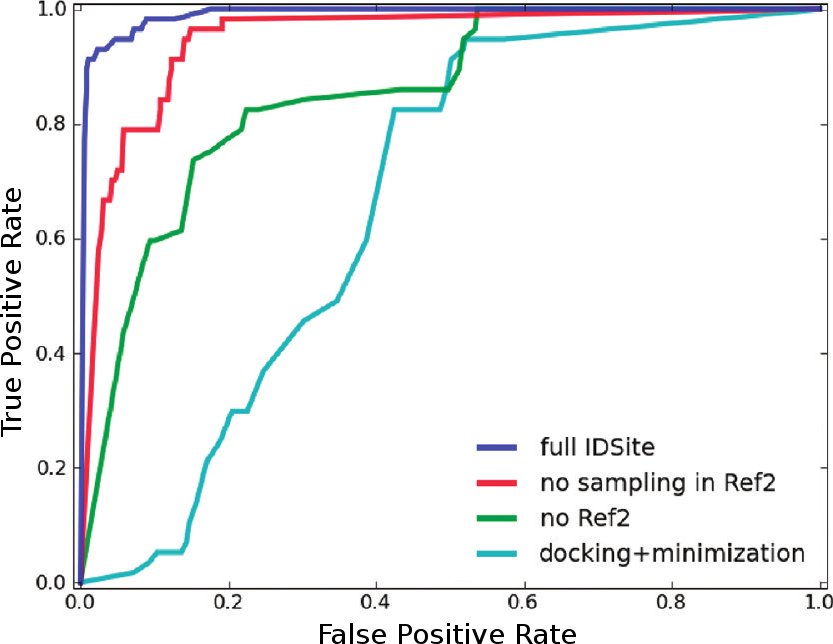
\includegraphics[width=0.5\textwidth]{figures/idsite/roc_sampling.png}
\caption{The effect of additional sampling on prediction of site of metabolism by P450.
The light blue series describes only performing the initial Glide docking stage followed by minimization.
The green series is obtained by using the set of structures obtained in the first minimization Monte Carlo sampling stage.
The red series is obtained by screening the structures obtained in the first sampling stage, and minimizing these structures using the constraints specified in Figures \ref{figure:second_sp2_constraints} and \ref{figure:second_sp3_constraints}.
The blue series makes use of the entire IDSite procedure.
The color scheme of these series corresponds to the colors of edges in Figure \ref{figure:idsite_overview}.}
\label{figure:idsite_roc_sampling}
\end{figure}
